\documentclass[11pt,onecolumn]{article}
\usepackage{amssymb, amsmath, amsthm,graphicx, paralist,algpseudocode,algorithm,cancel,url,color}
\usepackage{sectsty}
\usepackage{fancyvrb}
\usepackage{mathrsfs}
\usepackage{multirow}
\usepackage{hhline}
\usepackage{booktabs}
\usepackage[table]{xcolor}
\usepackage{tikz}
% \usepackage[framed,numbered,autolinebreaks,useliterate]{mcode}
\usepackage{listings}
\usepackage{enumitem}
\usepackage{cleveref}
\usepackage{tcolorbox}
\usepackage{mathtools}
\usepackage{pdfpages}
\usepackage{multicol}
\usepackage{lipsum}
\usepackage{mwe}
\graphicspath{ {./images/} }


\newcommand{\bvec}[1]{\mathbf{#1}}
\newcommand{\R}{\mathbb{R}}
\newcommand{\C}{\mathcal{C}}
\newcommand{\Rn}{\R^{n\times n}}
\newcommand{\Rmn}{\R^{m\times n}}
\newcommand{\Cn}{\C^{n\times n}}
\newcommand{\Cmn}{\C^{m\times n}}
\newcommand{\cO}{\mathcal{O}}
\newcommand{\ls}{\textsc{ls}}
\DeclareMathOperator{\Tr}{Tr}
\DeclareMathOperator{\trace}{trace}
\DeclareMathOperator{\diag}{diag}
\DeclareMathOperator*{\argmin}{arg\,min}
\DeclareMathOperator*{\argmax}{arg\,max}
\sectionfont{\Large\sc}
\subsectionfont{\sc}
\usepackage[margin=1 in]{geometry}
\DeclareMathOperator{\Tra}{Tr}

\DeclarePairedDelimiter{\abs}{\lvert}{\rvert}
\DeclarePairedDelimiter{\norm}{\lVert}{\rVert}
\DeclarePairedDelimiter{\innerproduct}{\langle}{\rangle}
\DeclarePairedDelimiter{\PAREN}{(}{)}
\DeclarePairedDelimiter{\BRACK}{[}{]}
\DeclarePairedDelimiter{\CURLY}{\{}{\}}

\newcommand{\bluebox}[1]{
  \begin{tcolorbox}[colback=blue!5!white,colframe=blue!75!black,boxrule=0.5pt,boxsep=0pt,left=6pt,right=16pt,top=4pt,bottom=4pt]
  #1
  \end{tcolorbox}   
}

\newcommand{\redbox}[1]{
  \begin{tcolorbox}[colback=red!5!white,colframe=red!75!black,boxrule=0.5pt,boxsep=0pt,left=6pt,right=16pt,top=4pt,bottom=4pt]
  #1
  \end{tcolorbox}
} 

\newcommand{\greenbox}[1]{
  \begin{tcolorbox}[colback=green!5!white,colframe=red!75!black,boxrule=0.5pt,boxsep=0pt,left=6pt,right=16pt,top=4pt,bottom=4pt]
  #1
  \end{tcolorbox}
} 

\begin{document}
\noindent
\textsc{\Large Numerical analysis: Project 1}\\
Instructor: Anil Damle\\
Due: March 10, 2025\\

By: Bodong Liu (bl576), Ryan Wu (rw645)
\bluebox{
\paragraph{Goal 1:}
Implement the Householder scheme for computing QR factorizations. Your QR factorization routine should take in a $n \times k$ matrix $B$ with $k\leq n$ and returns a $n\times k$ matrix $Q$ with orthonormal columns (or sufficient information to be able to apply it to a vector, e.g., the Householder vectors), and a $k\times k$ upper triangular matrix $R.$ Please demonstrate that your algorithm behaves as expected (this means both that you are getting a valid QR factorization as output and that it achieves the desired computational scaling). \textbf{Demonstrate that your implementation achieves the expected scaling and explain how you tested your implementation.}}

We perform the QR factorization using the Householder scheme, where given an input $B$ returns a set of orthonormal vectors $H_{vec}$ which can be used to reconstruct $Q$, and an upper triangular square matrix $R$ such that $QR=B$. The standard Householder scheme has an expected scaling of $O(mnl)$ where $l=\min \{m,n\}$, which in this case, $m\geq n$ for all inputs, thus there should be an expected scaling of $O(mn^2)$. 

At a high level, our algorithm (visible in code appendix), loops from $i=0...n$, and in each iteration of the loop, we find Householder reflection, which takes $O(m)$ operations, and perform the update $R[i:m,i:n] = R[i:m,i:n]-2v(v^\top R[i:m,i:n])$. This update consists of two vector-matrix multiplications, and then a matrix-matrix subtraction, which altogether requires $O(mn)$ operaions. Thus, each iteration has a time complexity of $O(mn)$, and it follows that the algorithm has an expected scaling of $O(mn^2)$. 

Next, we performed benchmarking to check the time complexity and scaling of our function. Below is the scaling on a log-log plot, specifically on tall-skinny matrices ($10n\times n$), which we see appears to scale around as expected at $O(mn^2)$.

$$
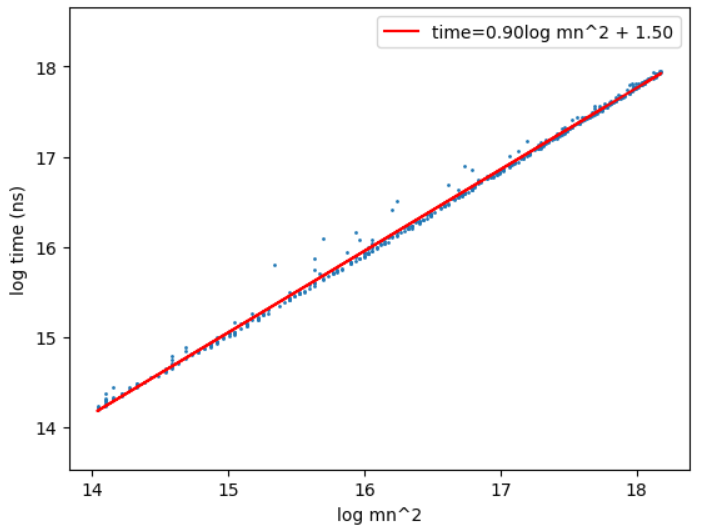
\includegraphics[scale=0.55]{./images/QRScaling.png}
$$
\newpage

We also benchmarked other cases: for square matrices, we have an expected time complexity of $O(n^3)$ because $m=n$. From the plot, it appears that there is indeed a cubic scaling factor. 
$$
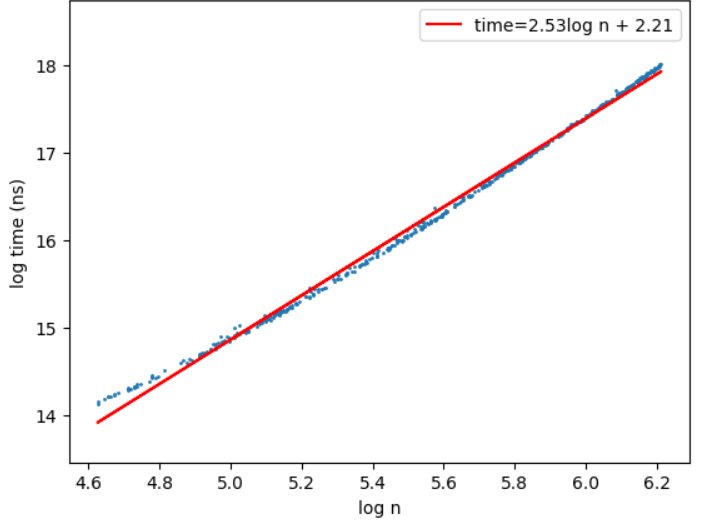
\includegraphics[scale=0.55]{./images/QRScaling_square.png}
$$

Below is the plot of our Householder algorithm on random $m\times n$ matrices, where $m\geq n$. Similarly, it is rather appropriately bounded by $O(mn^2)$.
$$
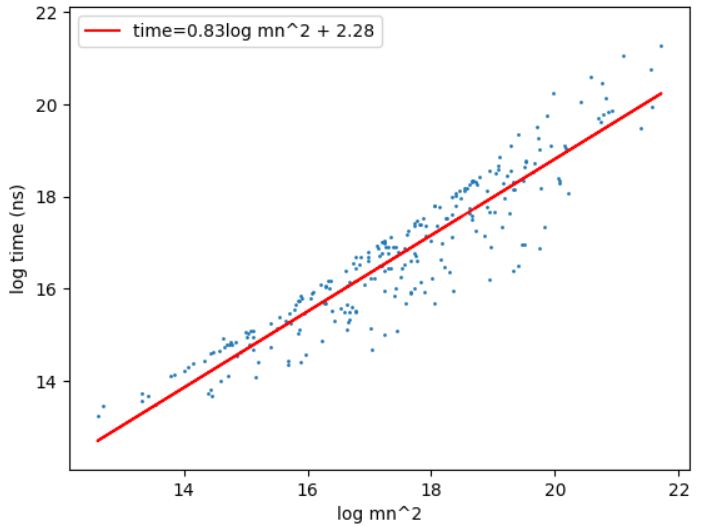
\includegraphics[scale=0.55]{./images/QRScaling_rectangular.png}
$$

To test our code, we created a script that generates 1000 random matrices $A$, where for each we explicitly compute $Q$ from the Householder vectors, then compare the product $QR$ against $A$. We also test that $R$ is indeed square upper triangular, and that $Q^\top Q=I$; $Q$ has orthonormal columns.
$$
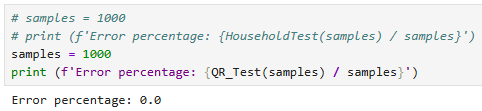
\includegraphics[scale=1]{./images/QRTest.png}
$$

\newpage
\bluebox{
\paragraph{Goal 2:} 
Using your $QR$ factorization, implement Algorithm 1. This is written as a matrix least squares problem, but think about the Frobenius norm and how you might be able to split it up into problems we know how to solve. \textbf{Please explain how you do this in the project report.} Practically, it is possible to then block some of these operations together for efficiency; you may take advantage of this if you wish.}
Given a QR factorization for $Z=QR$, and suppose $A-WZ^\top=B\in\mathbb R^{m\times n}$ 
\begin{align*}
  \norm{A-WZ^\top}_F^2&=\Tra \PAREN*{(A-WZ^\top)^\top (A-WZ^\top)}
  \\ &= \Tra \PAREN*{A^\top A} - 2\Tra \PAREN*{A^\top WZ^\top} + \Tra\PAREN*{ZW^\top WZ^\top}
\end{align*}

We wish to take the derivative with respect to $Z$. We observe the following:

\begin{align*}
  \nabla_W\Tra\PAREN*{A^\top A}&=0                      \\ 
  \nabla_W\Tra\PAREN*{2A^\top WZ^\top}&=-2AZ \\
  \nabla_W\Tra\PAREN*{ZW^\top WZ^\top}=\nabla_W\Tra\PAREN*{WZ^\top ZW^\top}&=2W Z^\top Z
\end{align*}

Setting the derivative to 0, we have:
\begin{align*}
  \nabla_Z\norm{A-WZ^\top}_F^2=0&=2WZ^\top Z-2AZ \\ 
  WZ^\top Z&= AZ \\
  Z^\top ZW^\top&=Z^\top A ^\top\\
  R^\top Q^\top QR W^\top&=R^\top Q^\top A^\top \\ 
  RW^\top&=Q^\top A^\top
\end{align*}

Thus, the $W$ that solves $RW^\top =Q^\top A^\top$ achieves the least squares minimum while holding $Z$ constant. Similarly, if we have a QR factorization $W=QR$, we have the least squares minimum while holding $W$ constant to be $RZ^\top=Q^\top A$. Since $R$ is upper triangular in both cases, we have an algorithm to solve for the argmin: use back substitution to solve the above systems for $W^\top$ and $Z^\top$. $Q^\top A$ can easily be calculated by applying the Householder vectors. Thus, we have the following algorithm:

\newpage 

\begin{algorithm}
  \caption{Alternating least squares, without regularization}
  \begin{algorithmic}[1]
    \State {\bf initialize} $W \in \R^{n_1 \times k}$, $Z \in \R^{n_2 \times k}$
      \While{not converged}
        \State $$Q_Z, R_Z \leftarrow (Z)$$
        \State $$Q_W, R_W \leftarrow (W)$$
        \State $$Z^\top \leftarrow R_W^{-1}Q_W^\top A$$ 
        \State $$W \leftarrow R_Z^{-1}Q_Z^\top A^\top$$ 
      \EndWhile
    \State {\bf return} $W$, $Z$
  \end{algorithmic}
\end{algorithm}

The Python implementation can be found in the appendix.\\

\newpage
\bluebox{
\paragraph{Goal 3:}
Using your implementation, load the file Cornell.csv which has an image stored in the matrix $C$ and try to compute the best rank 75 approximation of the image. Compare this with the result of the best rank 75 image from the SVD (you can use a built in routine to compute this), what do you observe qualitatively and quantitatively?}

The SVD approximation has a clearer and more detailed image, although just by a little. There is less ``noise" that is present in the white areas of the image. On the other hand, QR/ALS approximation was a bit blurrier and had noise in the ``white'' portions of the image. ALS approximation also improved (compared to itself) with more iterations and depending on the initialization. Quantitatively the SVD has the optimal/lowest norm possible. In terms of runtime, ALS ran for significantly longer, and seems to be less computationally efficients than directly computing the SVD solution.


\begin{figure}[H]
  \centering
  \begin{minipage}{0.45\textwidth}
    \centering
    
\includegraphics[width=0.9\textwidth]{./images/ALS.png}
    \caption{ALS approx}
  \end{minipage}\hfill
  \begin{minipage}{0.45\textwidth}
    \centering
    
\includegraphics[width=0.9\textwidth]{./images/SVD.png}
    \caption{SVD approx}
  \end{minipage}
\end{figure}

The code to generate these images can be located in the appendix at the end.

\newpage
\bluebox{
\paragraph{Question 1:}
Show that if we want to solve $$\min_x \|Ax-b\|_2^2 + \beta^2 \|x\|_2^2$$ we can instead solve 
\[
\min_x \left\|\begin{bmatrix}A \\ \beta I\end{bmatrix}x-\begin{bmatrix}b \\ 0\end{bmatrix}\right\|_2^2.
\]}

We observe the quantity that we want to minimize:
\begin{align*}
  \norm{Ax-b}_2^2+\beta^2\norm{x}_2^2 &= (Ax-b)^\top(Ax-b)+\beta^2x^\top x
  \\ &=x^\top A^\top Ax-b^\top Ax-x^\top A^\top b+b^\top b+\beta^2x^\top x
  \\ &=x^\top A^\top Ax+\beta^2 x^\top x - b^\top Ax - x^\top A^\top b+b^\top b
  \\ &= x^\top (A^\top A + \beta^2 I) x - (b^\top A + 0)x-x^\top (A^\top b + 0) + (b^\top b + 0)
  \\ &= x^\top \begin{bmatrix} A^\top & \beta I\end{bmatrix}\begin{bmatrix}A \\ \beta I\end{bmatrix} x - \begin{bmatrix}b^\top & 0\end{bmatrix}\begin{bmatrix}A \\ \beta I\end{bmatrix}x-x^\top \begin{bmatrix}A & \beta I\end{bmatrix} \begin{bmatrix}b \\ 0\end{bmatrix} + \begin{bmatrix}b^\top & 0\end{bmatrix}\begin{bmatrix}b \\ 0\end{bmatrix} 
  \\ &=\PAREN*{x^\top \begin{bmatrix} A^\top & \beta I\end{bmatrix} - \begin{bmatrix}b^\top & 0 \end{bmatrix}} \PAREN*{\begin{bmatrix} A \\ \beta I\end{bmatrix}x - \begin{bmatrix}b \\ 0 \end{bmatrix}}
  \\ &=\PAREN*{\begin{bmatrix} A \\ \beta I\end{bmatrix}x - \begin{bmatrix}b \\ 0 \end{bmatrix}}^\top \PAREN*{\begin{bmatrix} A \\ \beta I\end{bmatrix}x - \begin{bmatrix}b \\ 0 \end{bmatrix}}
  \\ &=\norm*{\begin{bmatrix} A \\ \beta I\end{bmatrix}x - \begin{bmatrix}b \\ 0\end{bmatrix}}^2_2
\end{align*}

Thus, since $\norm{Ax-b}_2^2+\beta^2\norm x_2^2=\norm*{\begin{bmatrix} A \\ \beta I\end{bmatrix}x - \begin{bmatrix}b \\ 0\end{bmatrix}}^2_2$, their minimums are the same, thus solving one is the same as solving the other problem.

\newpage
\bluebox{
\paragraph{Goal 4:}
Using your $QR$ factorization, implement Algorithm 2. From the first set of goals, you should have worked out how to split this up into solving many least squares problems. Now, you have to think about what size those problems are, and which entries of the matrices they involve. Given that, you can then leverage your $QR$ factorization and the preceding item to implement the algorithm. \textbf{Please explain how you do this in the project report.}}

\noindent The algorithm we implemented simplifies the problem into two quadratic problems that could be individually handled by QR factorization: \\

\noindent
Initialization:\\
We have the inputting matrix $A$ with shape $(n \times m)$, the rank $k$, and the regularization constant $\beta$. Initialize matrix $W$ $(n \times k)$, and matrix $Z$ $(m \times k)$ with random entries.\\

\noindent
Main Loop:\\
The algorithm iteratively estimates $W$ and $Z$ over a fixed number of iterations of the user's choice. At each iteration of the main loop, there are two loops that update $W$ and $Z$ respectively.


\noindent
 (a) Sub Loop for Updating $Z$ (Column Update)
\begin{enumerate}
\item For each column $j$ of $A$, the algorithm identifies the set of row indices where an observation exists by checking the mask.

\item If no observations are present on the column $j$, we set $Z[j, :]$ to 0 and skip to next iteration.

\item Otherwise, the algorithm forms a "local" sub-problem using $W_{\text{sub}}$, which is a subset of rows from $W$ where observations exist on the column $j$, and the algorithm forms $A_{\text{sub}}$, which holds the values of the observed entries in column $j$.
                $$W_{\text{sub}}=W[\text{observed, :}], A_{\text{sub}}=A[\text{observed}, j]$$
\item Then we can solve the regularized least squares problem as presented below:
$$\text{minimize }\|W_{\text{sub}}z - A_{\text{sub}}\|^2+\beta^2\|z\|^2$$
Which is equivalent of solving the below as shown by Question 1 by augmenting $W_{\text{sub}}$ with $\beta I$, and augmenting $A$ with zeros. This converts the problem into a least squares problem.

\item The system is solved by using QR factorization. More specifically, we obtain the $R$ matrix and the Householder vectors. Then we apply the Householder vectors the right hand side 
$
\begin{bmatrix}
    A_{\text{sub}} & 0
\end{bmatrix}^\top
$. Then we can easily solve the system.

\item The algorithm inserts the solution to the $j$-th row of $Z$, ie, $Z[j,:]$.
\end{enumerate}
(b) Sub Loop for Updating $W$ (Row Update)
\begin{enumerate}
 \item This sub loop is analogous to the column update but applied row-wise. 
 \item Depending on if there exists observations, we either set $W[i, :]$ to zeros, or update $W[i,:]$ using the rows from $Z$  ($Z_{\text{sub}}$) and actual values from $A$ ($A_{\text{sub}}$). 
 $$Z_{\text{sub}}=W[\text{observed, :}], A_{\text{sub}}=A[i, \text{observed}]$$
 \item The rest is the same operations with different inputs as the column update.
 (end of algorithm)
\end{enumerate}

\bluebox{
\paragraph{Goal 5:}
Using your implementation, load each of the image files in Image*.csv and associated masks Mask*.csv, where * is 1, 2, and 3. Each file contains an image and the associated mask file contains an image of the same size whose entries are 1 if the corresponding entry of $C$ is observed and 0 if it is unobserved (so it defines the set $\Omega$). The unknown entries of $C$ have been set arbitrarily and you should not access or use them (as the will adversely affect your results). Using Algorithm~\ref{alg:als2}, try and recover each of the underlying images. You now have some parameters to consider and we encourage exploration of their values. You should not have to go to $k$ larger than 75 for any of the examples, and good $\beta$ to try are between $10^{-2}$ and 1. Report the images you recover, and discuss what you observe.}

Effects of $\beta$:
A small regularization constant means weak penalization of large entries in the factor matrices. This can result in a closer fit to the observed data but may also amplify noise, potentially leading to an unstable approximation that overfits the observed pixels. A bigger $\beta$ imposes a harsher penalty, enforcing smaller norms on $W$ and $Z$. A large $\beta$ helps prevent overfitting and improves the stability of the solution by smoothing the reconstructed image. However, a very large $\beta$ might over do it and make the image too smooth for details to be observable. As we can see from the comparison of 3 image2.png generated on different $\beta$ values, the one generated with very small $\beta=0.01$ has observable artifacts running through the image horizontally and vertically. The one generated with very large $\beta=1$ does not have the issues of the low $\beta$ one, but the important details such as facial features and cloth folds are smoothed out, which we can see by a comparison with the image generated with $\beta=0.5$.

\begin{figure}[H]
  \centering
  \begin{minipage}{0.3\textwidth}
    \centering
    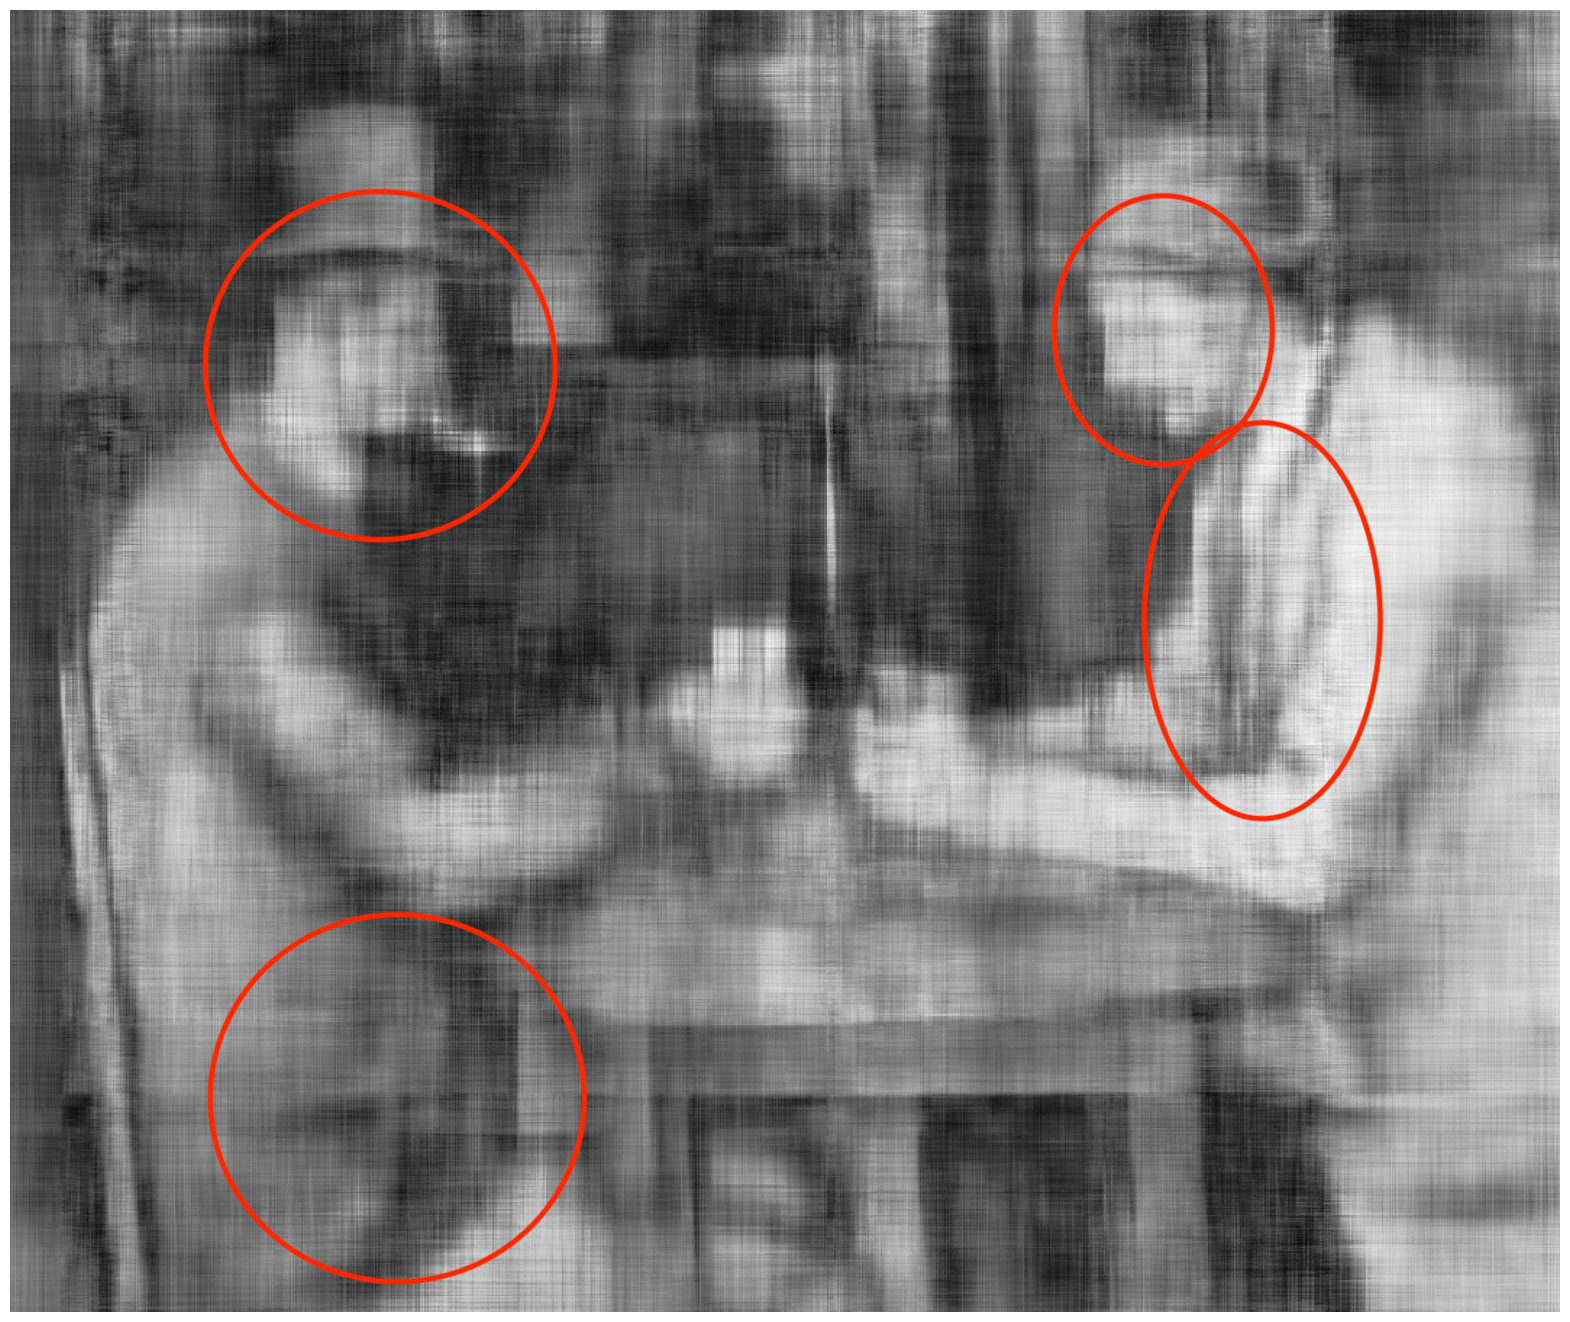
\includegraphics[width=1\textwidth]{./images/201.png}
    \caption{$\beta=1$, $k=30$, iter=5}
  \end{minipage}\hfill
  \begin{minipage}{0.3\textwidth}
    \centering
    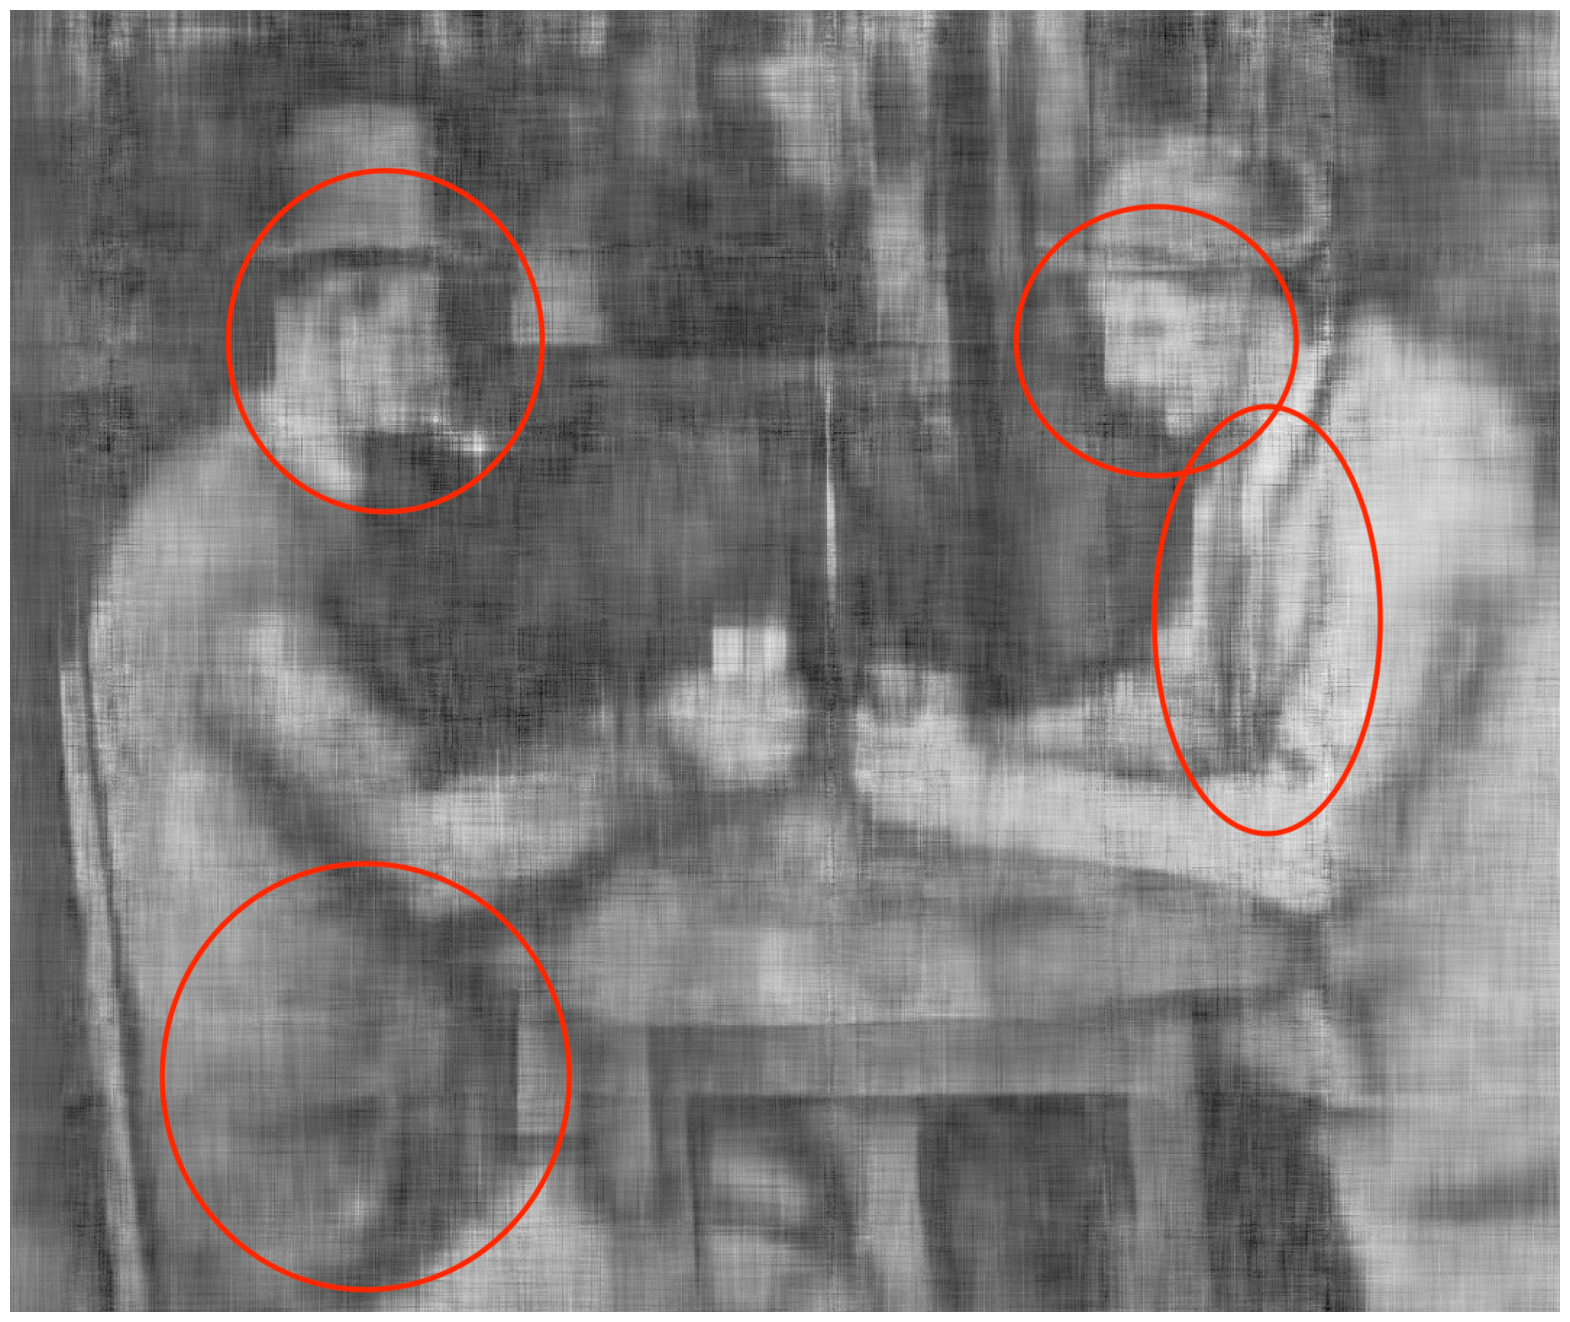
\includegraphics[width=1\textwidth]{./images/202.png}
    \caption{$\beta=0.5$, $k=30$, iter=5}
  \end{minipage}\hfill
  \begin{minipage}{0.3\textwidth}
    \centering
    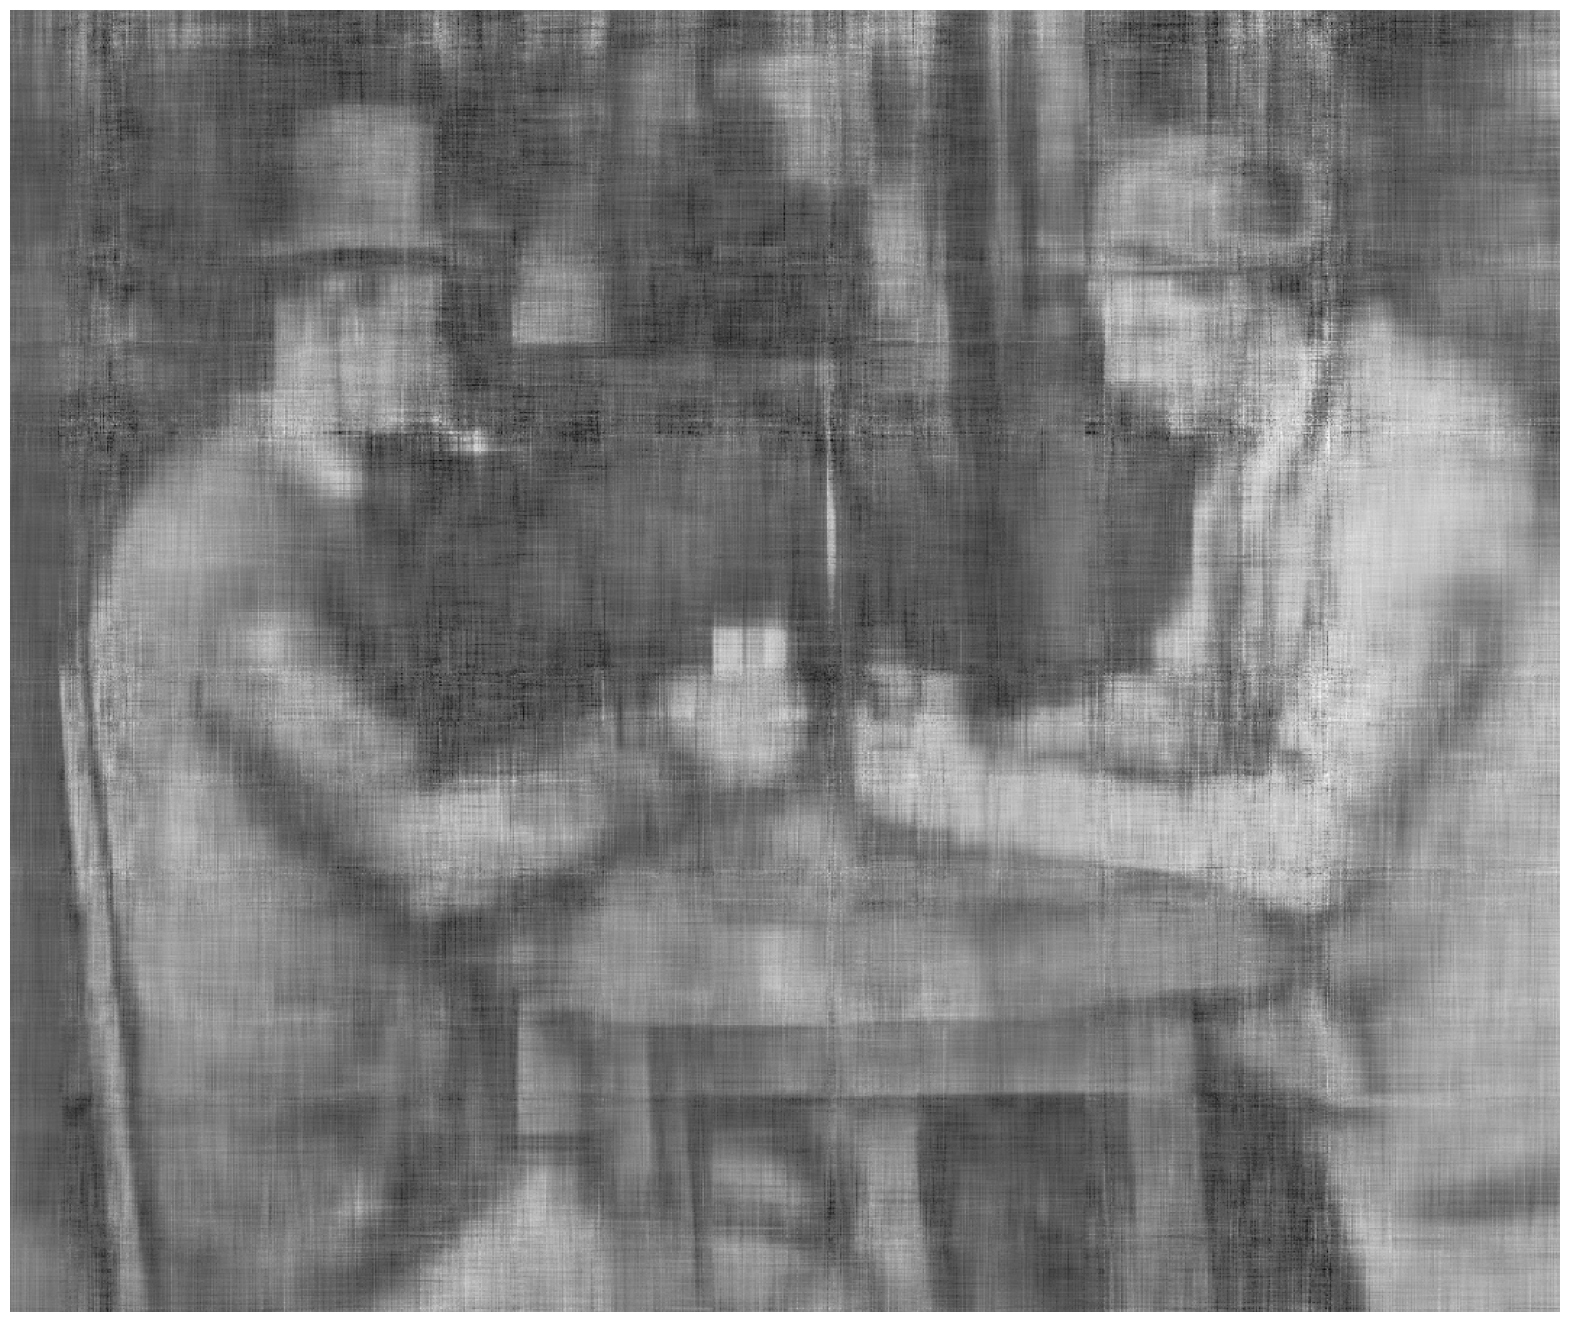
\includegraphics[width=1\textwidth]{./images/203.png}
    \caption{$\beta=0.01$, $k=30$, iter=5}
  \end{minipage}
\end{figure}

Effects of $k$:
A smaller rank forces a more compressed approximation that may oversimplify the image. This often results in a smooth or blurry reconstruction that neglects fine details, as the model lacks enough capacity to represent complex structures. A bigger $k$ allows the algorithm to capture more nuances and intricate details, leading to a reconstruction that is closer to the original image. However, if $k$ is too high, especially when the data is sparse or contaminated with noise, it may overfit the observed pixels, thereby including unwanted noise or artifacts. We can look at the comparison of the three images generated using different $k$ values ($k=10,20, 30$). It is quite obvious that as $k$ gets higher, more details are observable. Also note that a bigger $k$ is much more computationally heavy, by a quadratic factor.

\begin{figure}[H]
  \centering
  \begin{minipage}{0.3\textwidth}
    \centering
    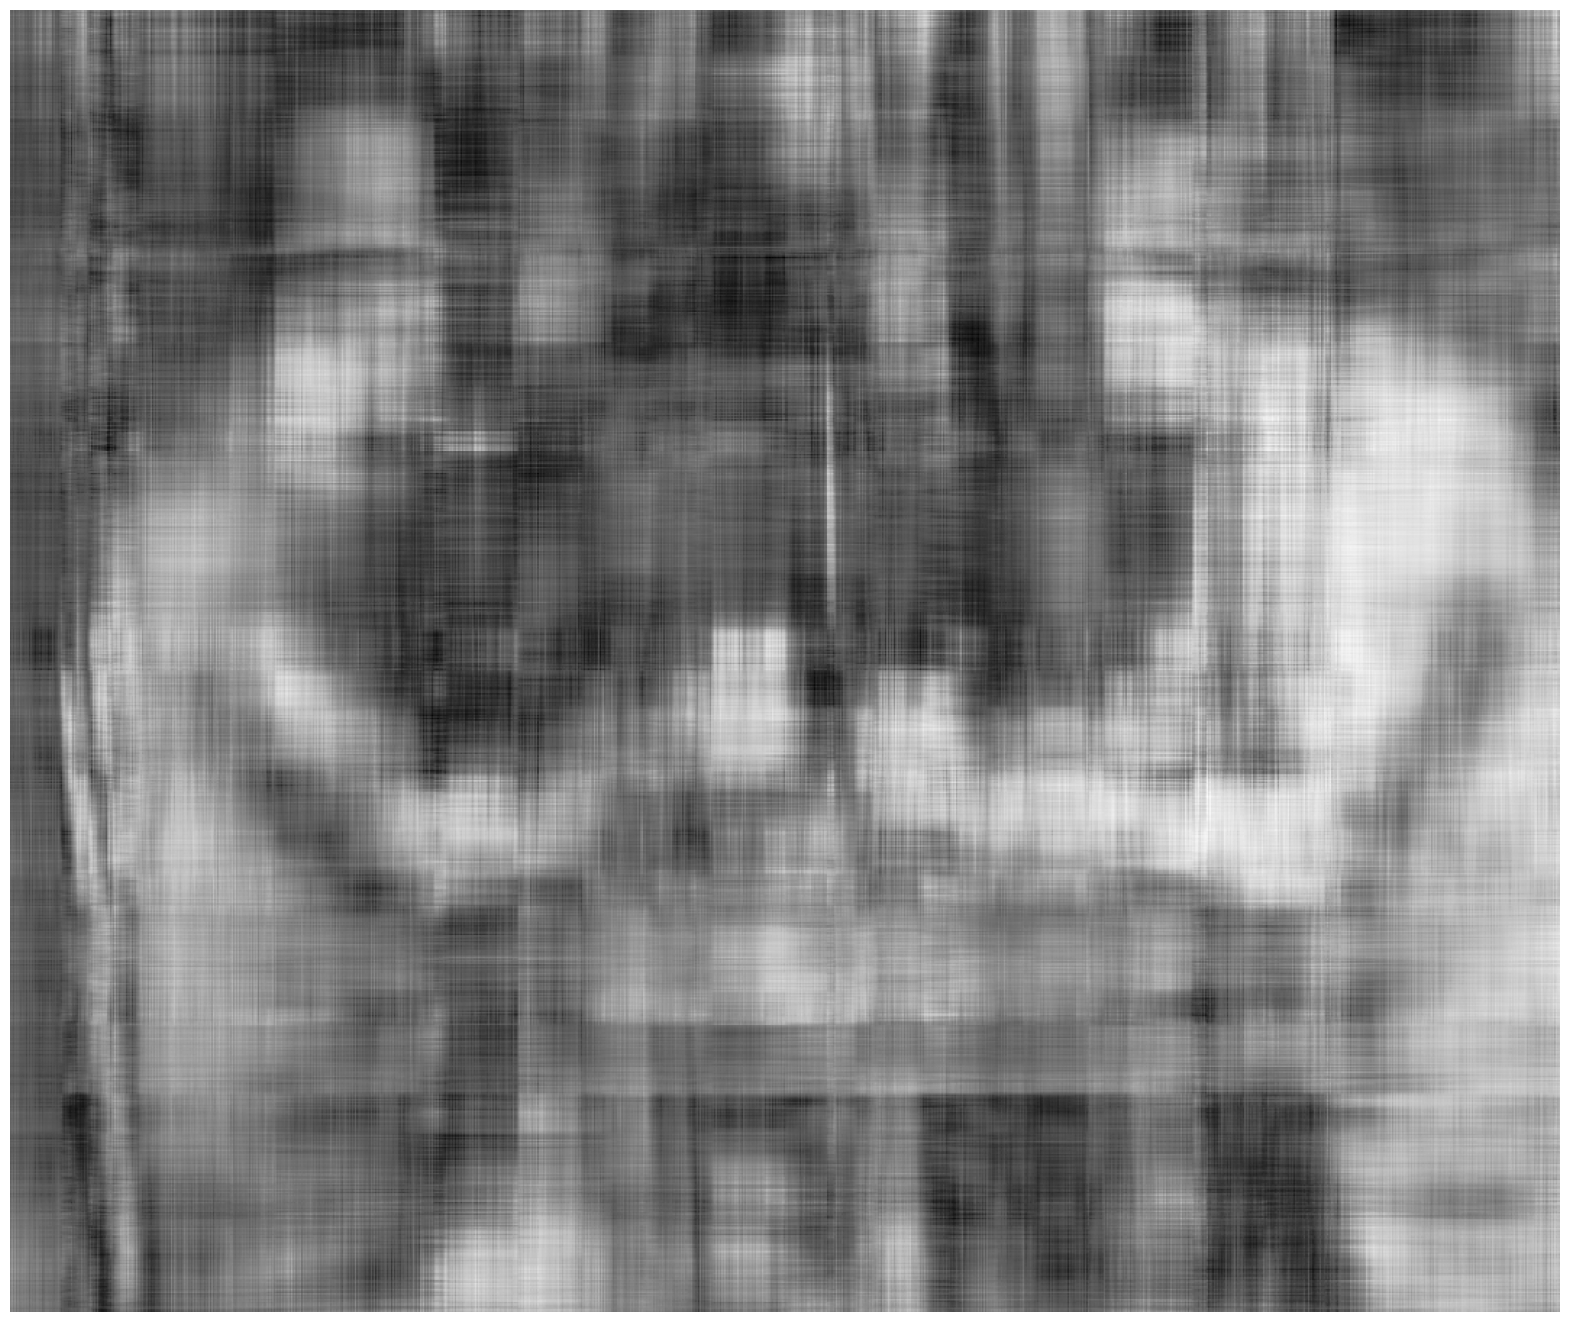
\includegraphics[width=1\textwidth]{./images/204.png}
    \caption{$\beta=0.6$, $k=10$, iter=5}
  \end{minipage}\hfill
  \begin{minipage}{0.3\textwidth}
    \centering
    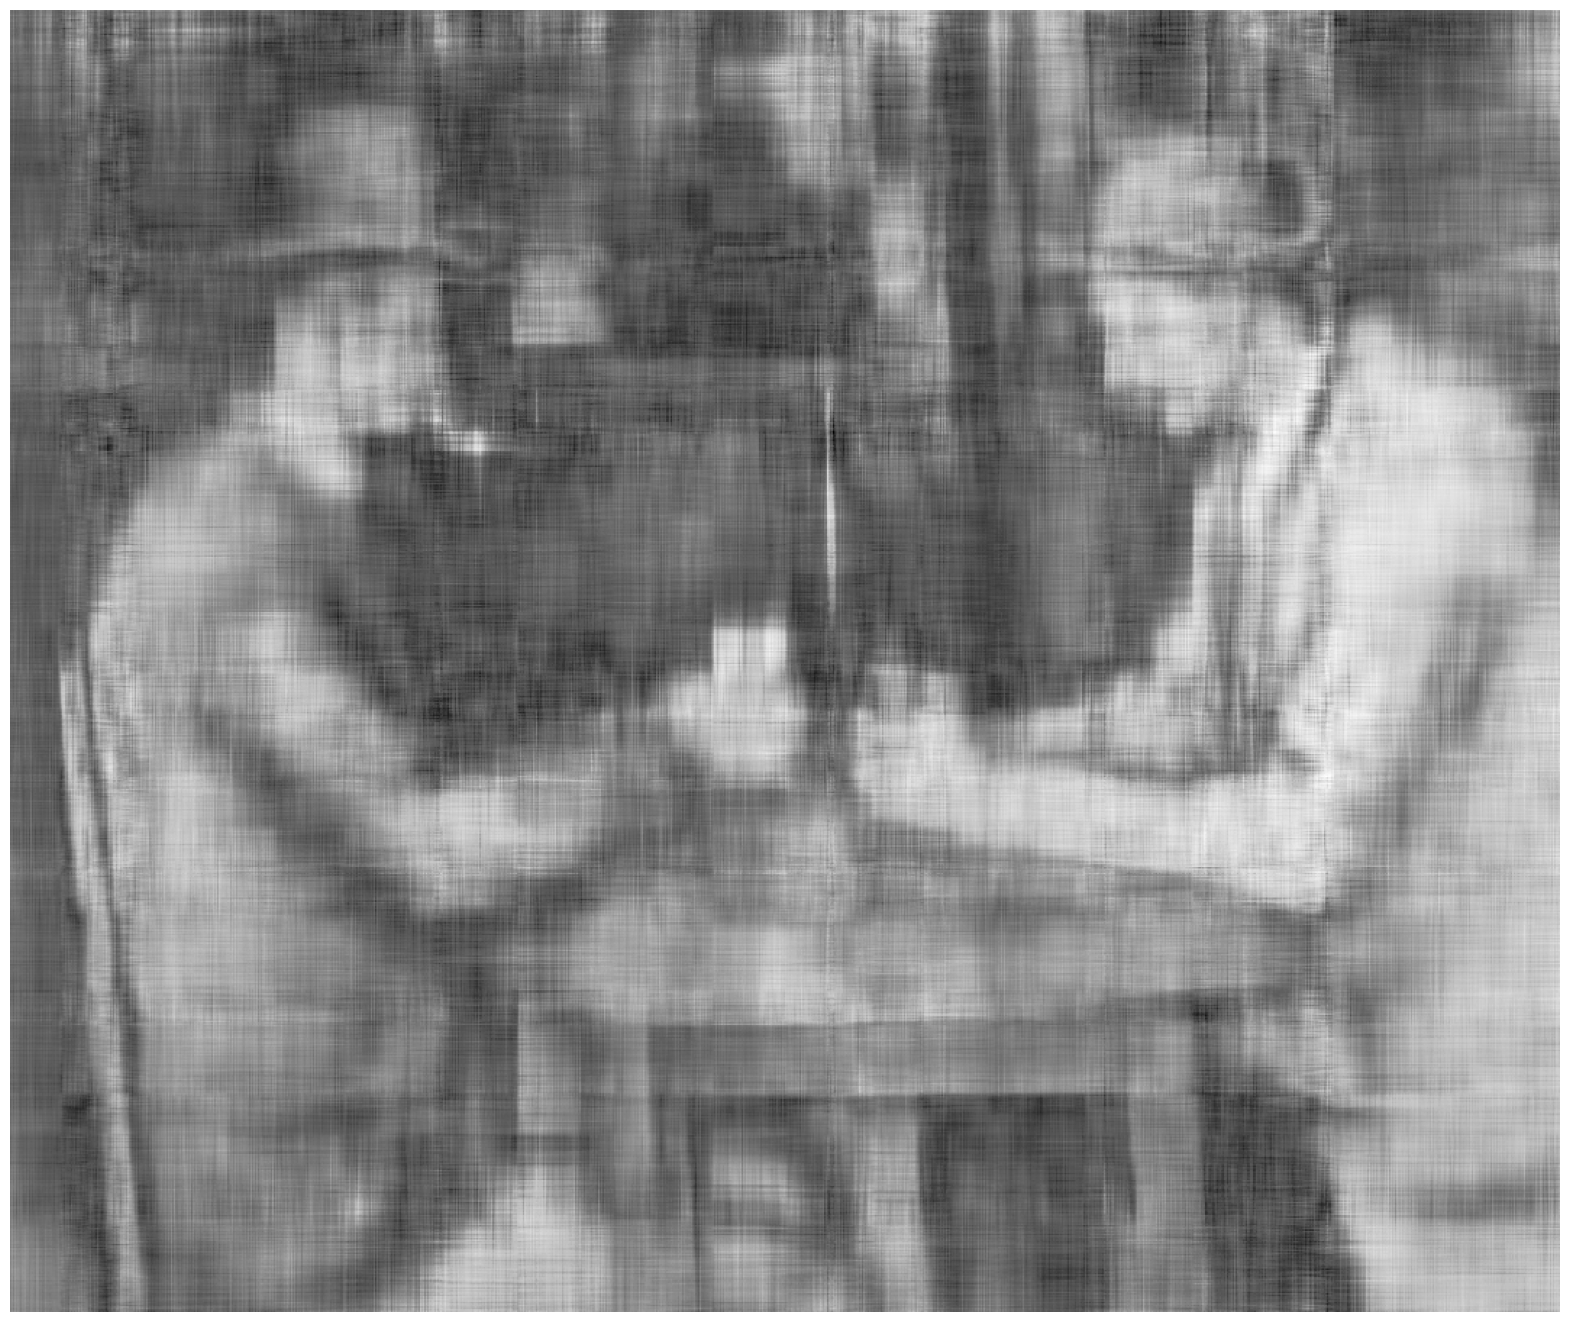
\includegraphics[width=1\textwidth]{./images/205.png}
    \caption{$\beta=0.6$, $k=20$, iter=5}
  \end{minipage}\hfill
  \begin{minipage}{0.3\textwidth}
    \centering
    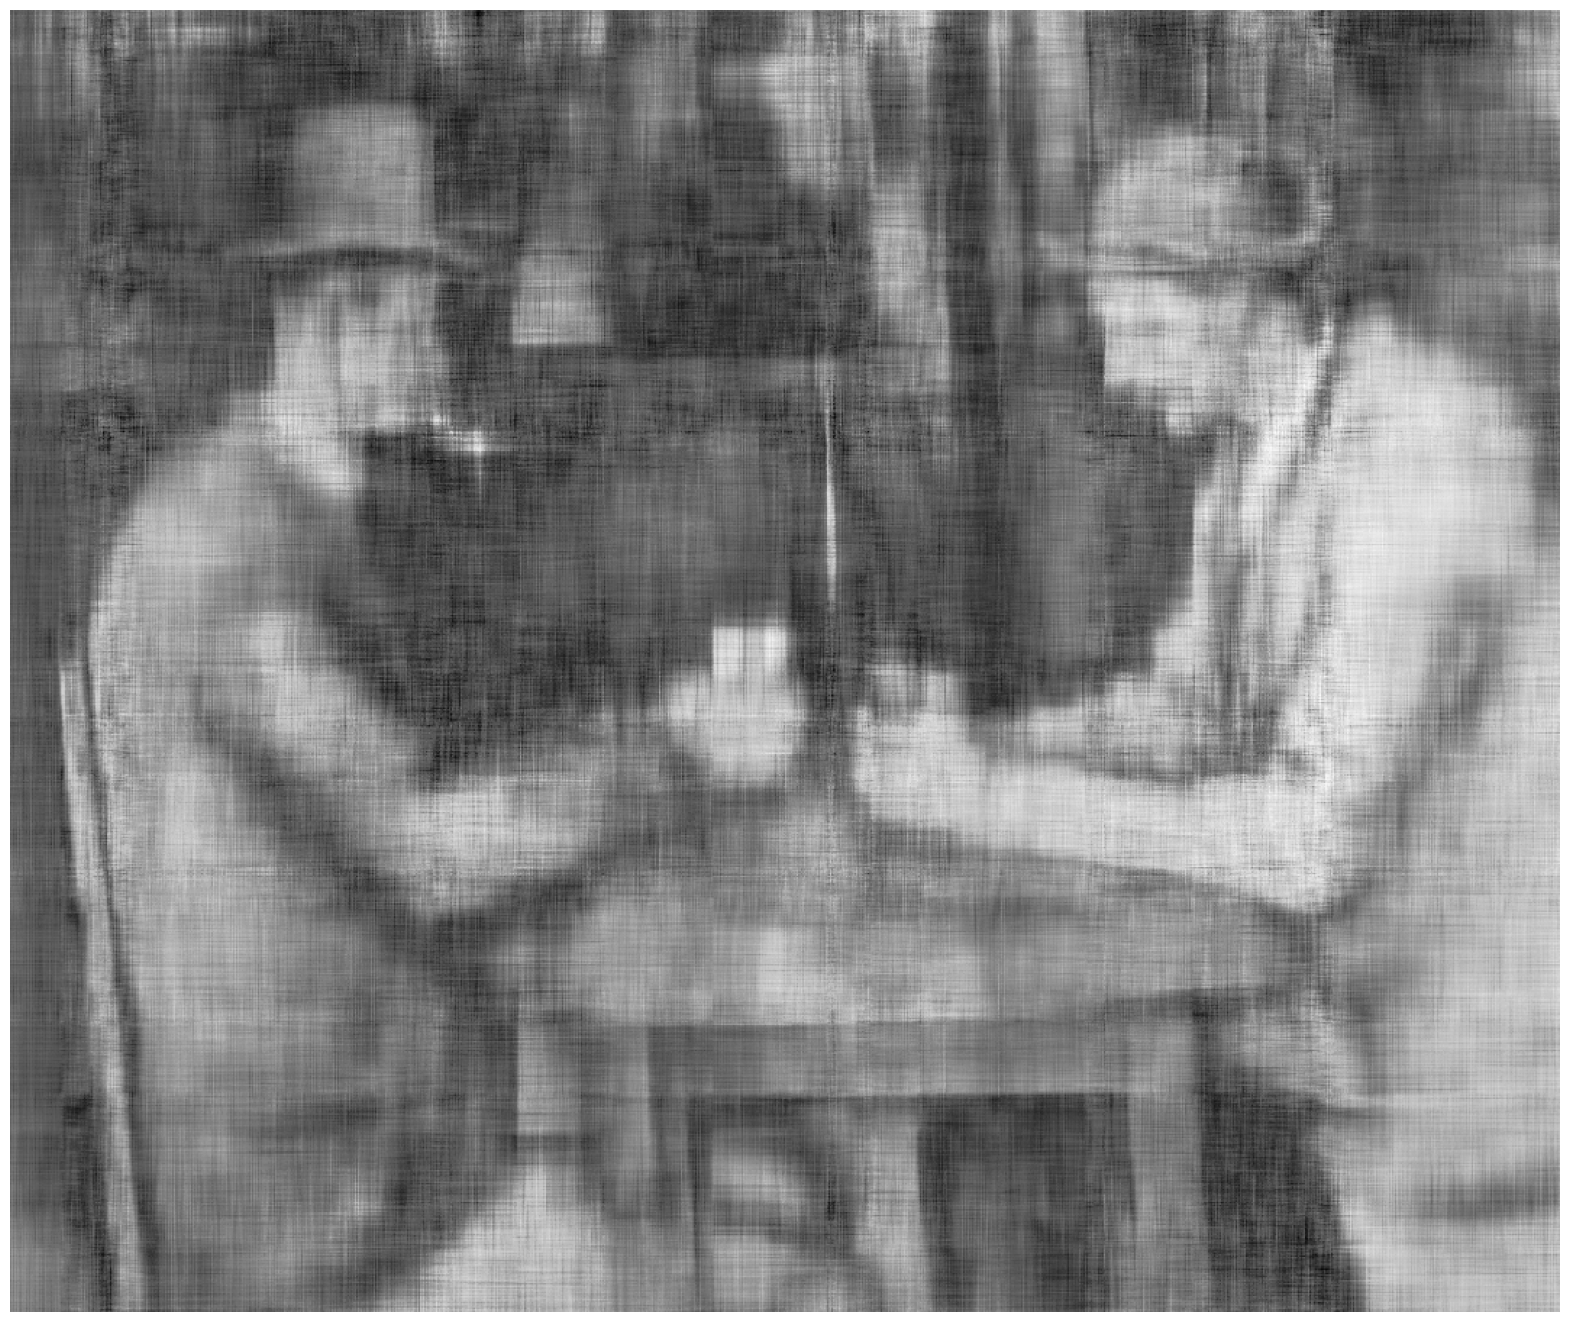
\includegraphics[width=1\textwidth]{./images/206.png}
    \caption{$\beta=0.6$, $k=30$, iter=5}
  \end{minipage}
\end{figure}

More examples and images are available in the appendix.

\includepdf[pages=-]{./code.pdf}

\end{document}
